% $Id: TimeMgr_obj4.tex,v 1.1 2002/08/18 22:43:36 eschwab Exp $

%\section{Object Model}

In Time Manager, all times are internally represented and operated on as
integer seconds and rational integer fractional seconds.  Specific date and
time formats are available to the user at the interface level, where
conversions are performed.  So the user gets/sets Time Manager's TimeIntervals
and TimeInstants in familiar units of year, month, day, hour, minutes,
seconds, and sub-seconds in their various required combinations.  Figure 4
shows an example of a user's ESM component quering its clock for the current
time in (YR, MM, DD, H, M, S) format.  First the model invokes the
Get\_YR\_MM\_DD\_H\_M\_S() method on its clock's current time, CurrTime.  Next,
internally (transparent to the user), CurrTime invokes the ConvertToDate()
method on its associated calendar, Gregorian.  Gregorian, in turn, performs
the requisite conversion of CurrTime's internal representation of time (integer
seconds and fractional seconds) to a Gregorian date.  Note that the calendar
object is a single instance shared among all TimeInstants, as previously shown
in Figures 1 and 2.

\begin{center}
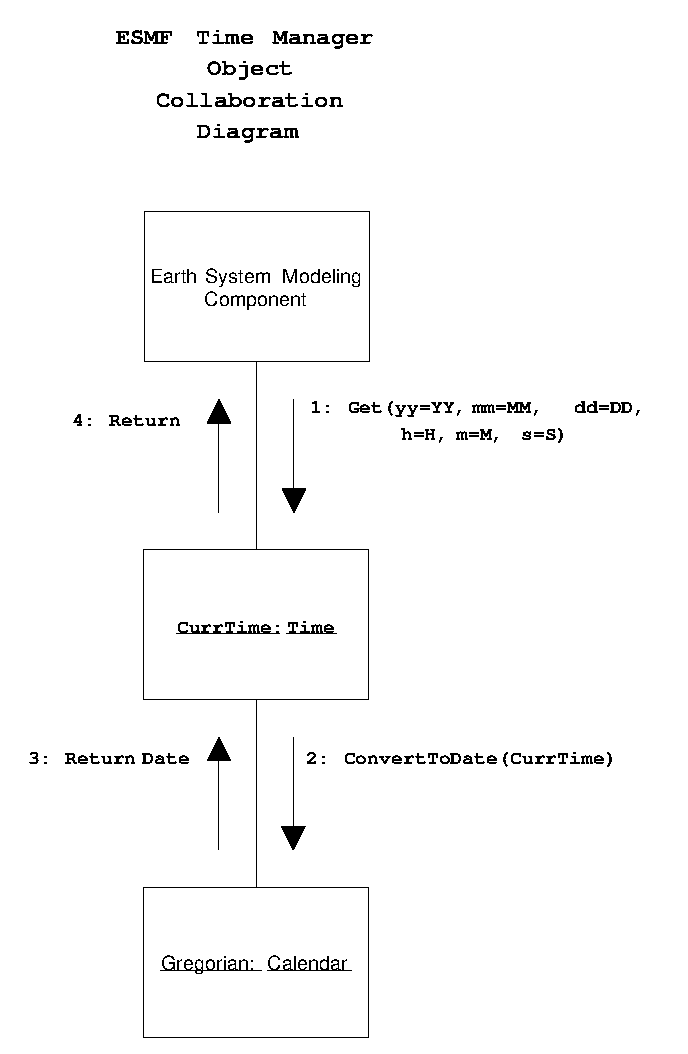
\includegraphics{TimeMgrOCD2.EPS}
   
Figure 4.  ESMF Time Manager Convert to Date Scenario
   
\end{center}
